%!TEX root = ../hutbthesis_main.tex

\chapter{仿真性能表现与问题分析}

\section{仿真测试环境搭建}

为保证实验公平性、可重复性、可对比性，搭建统一高性能测试环境，如表6所示。

\begin{longtable}[]{@{}
  >{\raggedright\arraybackslash}p{(\columnwidth - 2\tabcolsep) * \real{0.2171}}
  >{\raggedright\arraybackslash}p{(\columnwidth - 2\tabcolsep) * \real{0.7829}}@{}}
\caption{仿真测试硬件配置参数表}\\
\toprule\noalign{}
\begin{minipage}[b]{\linewidth}\raggedright
硬件类型
\end{minipage} & \begin{minipage}[b]{\linewidth}\raggedright
型号与参数
\end{minipage} \\
\midrule\noalign{}
\endhead
\bottomrule\noalign{}
\endlastfoot
处理器 & Intel Core i9-12900K（16 核 24 线程） \\
内存 & 64GB DDR5 4800MHz \\
显卡 & NVIDIA RTX 4090 24GB \\
硬盘 & 2TB NVMe SSD \\
操作系统 & Windows 10 专业版 64 位 \\
网络 & 千兆以太网 \\
\end{longtable}

注：(1)硬件环境全程固定，保证所有实验结果可对比；(2)配置满足大规模集群仿真算力需求。

软件环境采用固定版本，避免版本差异影响实验结果，如表7所示。

\begin{longtable}[]{@{}
  >{\raggedright\arraybackslash}p{(\columnwidth - 4\tabcolsep) * \real{0.2250}}
  >{\raggedright\arraybackslash}p{(\columnwidth - 4\tabcolsep) * \real{0.2048}}
  >{\raggedright\arraybackslash}p{(\columnwidth - 4\tabcolsep) * \real{0.5702}}@{}}
\caption{软件环境版本信息表}\\
\toprule\noalign{}
\begin{minipage}[b]{\linewidth}\raggedright
软件名称
\end{minipage} & \begin{minipage}[b]{\linewidth}\raggedright
版本号
\end{minipage} & \begin{minipage}[b]{\linewidth}\raggedright
用途
\end{minipage} \\
\midrule\noalign{}
\endhead
\bottomrule\noalign{}
\endlastfoot
Unity & 2021.3.15f1 & 仿真场景构建与环境渲染 \\
AirSim & 1.8.1-dev & 无人机集群核心仿真平台 \\
Visual Studio & 2022 & C++ 源码编译、工程构建与调试 \\
Python & 3.9 & 自动化测试、集群控制与数据采集 \\
ROS & Noetic & 协同算法部署与多机通信接口 \\
WPA & 10.0.19041 & Windows 平台性能追踪与瓶颈分析 \\
\end{longtable}

注：(1)所有软件版本固定，避免版本差异带来实验误差；(2)工具链用于源码修改与性能监测。

部署流程：

1.安装Unity引擎与AirSim插件；

2.编译AirSim C++源码生成Unity插件；

3.搭建多无人机仿真场景；

4.配置Python环境与AirSim API；

5.安装性能分析工具。

基于Unity引擎构建标准化仿真场景，具体类型如下图图9所示：

（1）场景类型

室外空地+简易建筑，无复杂渲染干扰；

（2）无人机型号

多旋翼Iris无人机；

（3）初始状态

均匀分布，悬停等待指令；

（4）控制方式

Python API批量生成、批量控制、批量采集数据。

\begin{figure}[H]
\centering

\includegraphics[width=0.88\linewidth,height=0.68\textheight,keepaspectratio]{images/image12.png}
\caption{多无人机集群仿真场景示意图}
\label{fig:09}
\end{figure}

场景支持1\textasciitilde100架无人机动态生成，提供悬停、编队、移动、避障等基础控制指令，支持帧率、时延、CPU占用等数据实时输出。具体实景演示如图所示：

\begin{figure}[H]
\centering
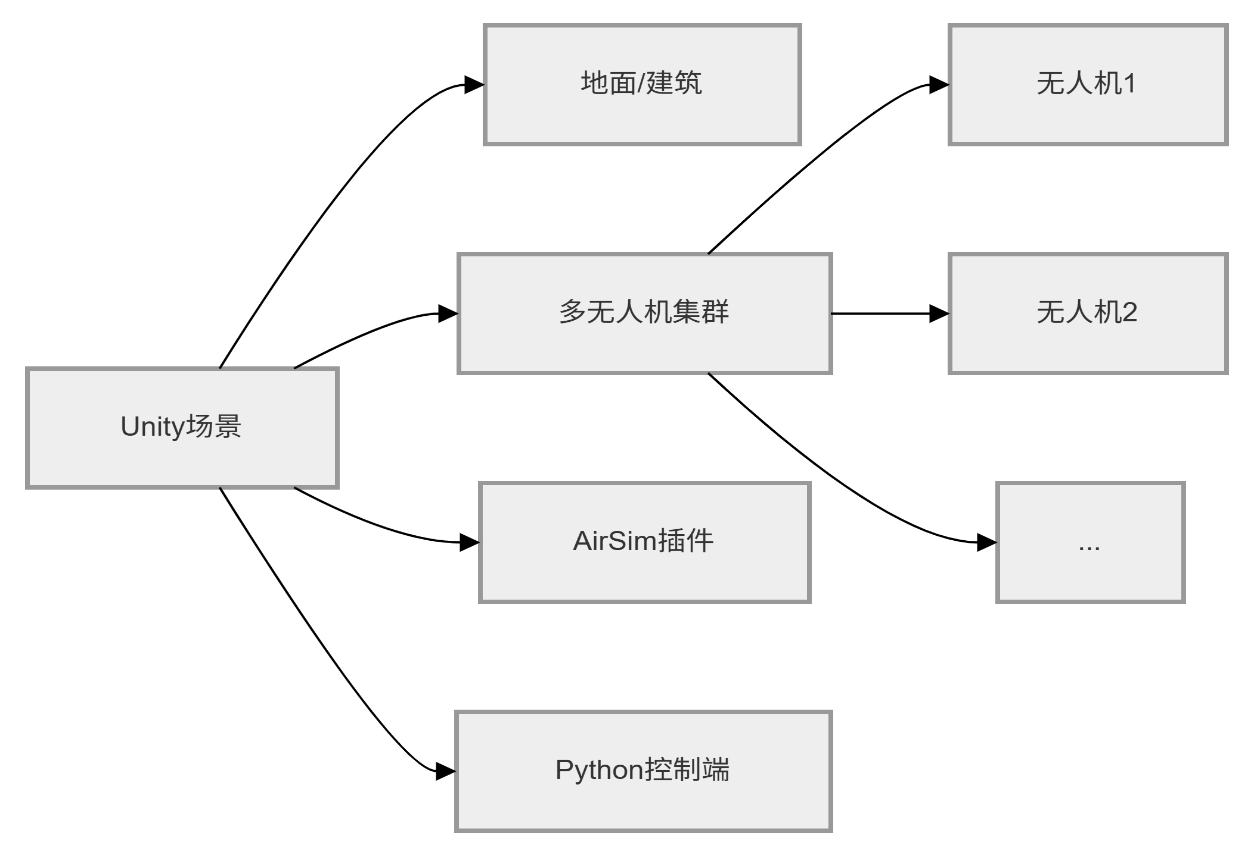
\includegraphics[width=0.88\linewidth,height=0.68\textheight,keepaspectratio]{images/image13.jpeg}
\caption{无人机3D场景全景图}
\label{fig:10}
\end{figure}

\section{不同规模集群下的仿真性能观测}

以无人机数量为变量，测试1\textasciitilde30架仿真帧率，结果如表5与图10所示。

\begin{longtable}[]{@{}
  >{\raggedright\arraybackslash}p{(\columnwidth - 8\tabcolsep) * \real{0.1602}}
  >{\raggedright\arraybackslash}p{(\columnwidth - 8\tabcolsep) * \real{0.1383}}
  >{\raggedright\arraybackslash}p{(\columnwidth - 8\tabcolsep) * \real{0.2180}}
  >{\raggedright\arraybackslash}p{(\columnwidth - 8\tabcolsep) * \real{0.2477}}
  >{\raggedright\arraybackslash}p{(\columnwidth - 8\tabcolsep) * \real{0.2357}}@{}}
\caption{不同规模集群仿真基础性能表}\\
\toprule\noalign{}
\begin{minipage}[b]{\linewidth}\raggedright
无人机数量
\end{minipage} & \begin{minipage}[b]{\linewidth}\raggedright
平均 FPS
\end{minipage} & \begin{minipage}[b]{\linewidth}\raggedright
平均时延（ms）
\end{minipage} & \begin{minipage}[b]{\linewidth}\raggedright
CPU 总占用（\%）
\end{minipage} & \begin{minipage}[b]{\linewidth}\raggedright
内核态占比（\%）
\end{minipage} \\
\midrule\noalign{}
\endhead
\bottomrule\noalign{}
\endlastfoot
1 & 62 & 8 & 12 & 18 \\
5 & 58 & 12 & 28 & 22 \\
10 & 45 & 24 & 47 & 31 \\
15 & 28 & 46 & 68 & 42 \\
20 & 12 & 98 & 89 & 58 \\
25 & 6 & 186 & 97 & 67 \\
30 & 3 & 292 & 99 & 72 \\
\end{longtable}

注：(1)数据为3次重复实验平均值；(2)20架以上出现性能断崖，内核占比过高为主要原因。

\begin{figure}[H]
\centering

\includegraphics[width=0.88\linewidth,height=0.68\textheight,keepaspectratio]{images/image14.png}
\caption{不同无人机数量帧率变化曲线图}
\label{fig:11}
\end{figure}

观测结论：

在1\textasciitilde10架时：FPS稳定，时延低，性能良好；

在10\textasciitilde20架时：性能快速下降；

当20架以上：FPS断崖式下跌，时延激增，CPU满负载，内核态占比超过70\%，仿真基本不可用。

测试不同规模下指令响应时延\textsuperscript{{[}3{]}{[}4{]}}，包括指令发送、接收、执行、状态反馈全流程，结果如图11所示。

\begin{figure}[H]
\centering

\includegraphics[width=0.88\linewidth,height=0.68\textheight,keepaspectratio]{images/image15.png}
\caption{仿真时延随集群规模变化趋势图}
\label{fig:12}
\end{figure}

时延增长呈现指数级特征，20架以上远超实时仿真要求（$\leq$50ms），导致控制指令堆积、无人机动作滞后、编队失序、仿真失步。

长期观测（30分钟）结果：

1\textasciitilde10架：内存稳定、GPU占用低、无卡顿、无崩溃；

15\textasciitilde20架：内存缓慢上升、GPU占用增加、偶发卡顿；

25\textasciitilde30架：内存暴涨、GPU满负载、频繁卡顿、仿真失步、概率性崩溃。

资源占用异常并非源于渲染负载，而是CPU线程调度与内核态开销，证明性能瓶颈在软件层而非硬件层。

\section{仿真性能下降的成因分析}

使用WPA捕获CPU占用数据，分析结果：

（1）用户态CPU占用

随无人机数量增加平稳上升；

（2）内核态CPU占用

呈指数级上升，20架以上占比超过70\%；

（3）线程状态

大量线程处于就绪/等待状态，频繁切换。

典型数据：30架无人机仿真时，总CPU占用99\%，其中内核态72\%，用户态仅27\%。说明CPU资源几乎全部浪费在内核态切换与调度上，而非仿真计算。

\begin{figure}[H]
\centering

\includegraphics[width=0.88\linewidth,height=0.68\textheight,keepaspectratio]{images/image16.png}
\caption{CPU内核态/用户态占比分布图}
\label{fig:13}
\end{figure}

AirSim大规模仿真性能下降，最直接的体现就是内核态占比过高。其根源在于大量线程频繁地执行系统调用，像sleep(0)、yield这些操作，进而触发了高频的用户态/内核态切换。为了能够精准找出AirSim原生集群仿真性能损耗的根源，在这一节里，使用Windows
Performance
Analyzer（WPA）工具来对仿真进程进行全量调用栈捕获、热点函数统计分析。结果表明，系统级线程调度相关的函数在CPU执行时间里占据了主要比例，其中Sleep、SwitchToThread、Yield等高频系统调用的耗时占比要高于业务逻辑函数。

随着无人机数量的增多，高频系统调用、大量冗余线程一同引发了调度风暴、内核态开销剧增、上下文切换频繁等系统性问题，最终在大规模集群仿真里出现了FPS大幅下降、时延飙升、CPU资源耗尽这样灾难性的性能退化。在基于Intel超线程架构CPU（16核24线程）的实验环境里，AirSim原生线程模型的性能缺陷被进一步放大。当集群中无人机数量超过CPU物理核心数（16核）以后，系统线程调度压力急剧上升，线程间资源竞争呈现出指数级加剧的趋势。大量线程依靠sleep(0)和yield来实现空转等待，线程会不断主动让出CPU时间片并触发重新调度，使得操作系统内核一直处于高频率调度状态。随着线程数量不断增多，大量就绪线程同时竞争有限的CPU时间片，最终引发严重的调度风暴，致使系统上下文切换频率从常规状态的每秒数万次快速攀升至每秒数百万次。


\begin{equation}
	C=N_{thread}\times f_{yield}\text{\footnotemark[1]}
	\label{eq:syscall-time}
\end{equation}
\footnotetext[1]{上下文切换次数与线程数量、线程主动让出频率成正比。AirSim
	原生sleep(0)使\emph{f}\textsubscript{yield}极高，规模扩大后出现调度风暴。}
高频切换进一步破坏CPU缓存局部性，造成缓存命中率持续下降、缓存频繁刷新失效，进而引发内存访问延迟显著增加、有效计算比重持续降低，使整个集群仿真系统陷入严重的性能恶化。

\section{关键影响因素的归纳与实验验证}

经定位，AirSim大规模集群仿真存在四大核心瓶颈：

（1）线程模型不合理

每机一线程，数量无限制，无池化管理；

（2）等待机制低效

使用sleep(0)与yield，高并发下触发高频切换；

（3）内核态开销过高

系统调用频繁，占比超过70\%；

（4）无调度优化

无负载均衡、无亲和性绑定、无超线程适配。

通过实验测试、对源码进行深入剖析可以发现，AirSim在大规模无人机集群仿真场景之下存在着四大核心性能瓶颈，具体情况如下。

首先是线程模型设计不够合理，它采用的是``单机一线程''的原生实现方式，线程数量会随着无人机规模呈现线性增长，并且没有上限约束，同时也没有引入线程池复用、动态创建销毁等轻量化管理机制，这使得系统线程资源出现严重冗余。其次是线程等待与同步机制效率较低，它默认使用sleep(0)与yield组合来实现空转等待，在高并发集群场景中会强制触发高频线程调度，进而引发大量无效切换、调度开销。最后是内核态运行开销占比过高，线程调度、系统调用等内核操作占用了大量CPU资源，内核态CPU占比最高能够达到70\%以上，有效业务计算资源被严重挤压。没有进行CPU亲和性绑定与核心隔离工作，也没有对超线程架构进行适配处理，这使得硬件资源利用率处于较低水平。

为了精准确定、验证大规模集群仿真性能出现退化现象的核心原因，本节设计了多组对照式控制变量实验。具体做法是逐一改变关键影响因素，同时观察性能变化状况，凭借此来实现瓶颈根源的量化验证。对超线程开关、等待机制类型、线程数量上限展开实验，实施单一变量控制。实验结果显示，关闭CPU超线程后，集群仿真性能有一定程度的回升，不过当无人机数量超过20架时，性能仍会出现大幅下跌的状况，这表明超线程并非导致瓶颈的决定性因素。把原生实现里的sleep(0)忙等方式替换成阻塞式sleep\_for等待策略后，系统上下文切换、内核态开销明显变小，整体仿真帧率和时延性能都获得了一定程度的改善，这直接验证了低效等待机制是影响集群性能的关键因素。通过人为限制最大并发线程数量，防止线程无节制地膨胀，仿真的稳定性和吞吐量有显著提高，这充分证实了线程模型不合理是致使大规模场景性能恶化的核心因素。经过对多组对照实验结果进行综合分析后可以明确得出，AirSim原有的线程架构、同步等待机制，是导致其在大规模无人机集群仿真中性能大幅下降的根本所在。。

\section{本章小结}

通过搭建标准化测试环境，基本复现AirSim大规模集群仿真性能问题，并通过专业工具深度定位瓶颈根源即线程模型不合理、等待机制低效、内核态开销过高、调度风暴。明确优化靶点与方向，为后续优化以及对比方案提供坚实依据。
